\section{Benchmark Characterization}
\Secl{results}

The released dataset contains 9,415 Lean 4 formalization challenges derived from 2,772 unique Python property-based tests, produced by two pipeline runs (\texttt{feb03}: 5,979 samples, Claude Sonnet; \texttt{apr08}: 3,436 samples, Claude Sonnet 4.6). Each unique PBT has between 1 and 15 formalizations. Among PBTs with multiple formalizations, 65\% have no single dominating attempt: for each formalization in the group there exists another that scores higher on at least one sub-metric of Equation~\ref{eq:faithfulness}. In practice this means, for example, that the attempt with the best assertion coverage may have worse parameter coverage than a sibling; keeping all formalizations and flagging the best one with \texttt{is\_canonical} therefore captures strictly more information than retaining only the top-scoring attempt.

\subsection{Translation Quality}

We evaluate translation quality using \emph{structural faithfulness} (Equation~\ref{eq:faithfulness}), a composite metric defined in \Secr{pipeline}. Figure~\ref{fig:structural_faithfulness} shows the distribution of the overall score and the mean of each sub-score across the dataset. The overall faithfulness distribution exhibits a clear mode above 0.5, indicating that the majority of translations preserve the essential structure of the source PBT, though a long tail of lower-quality translations remains.

\begin{figure}[t]
  \centering
  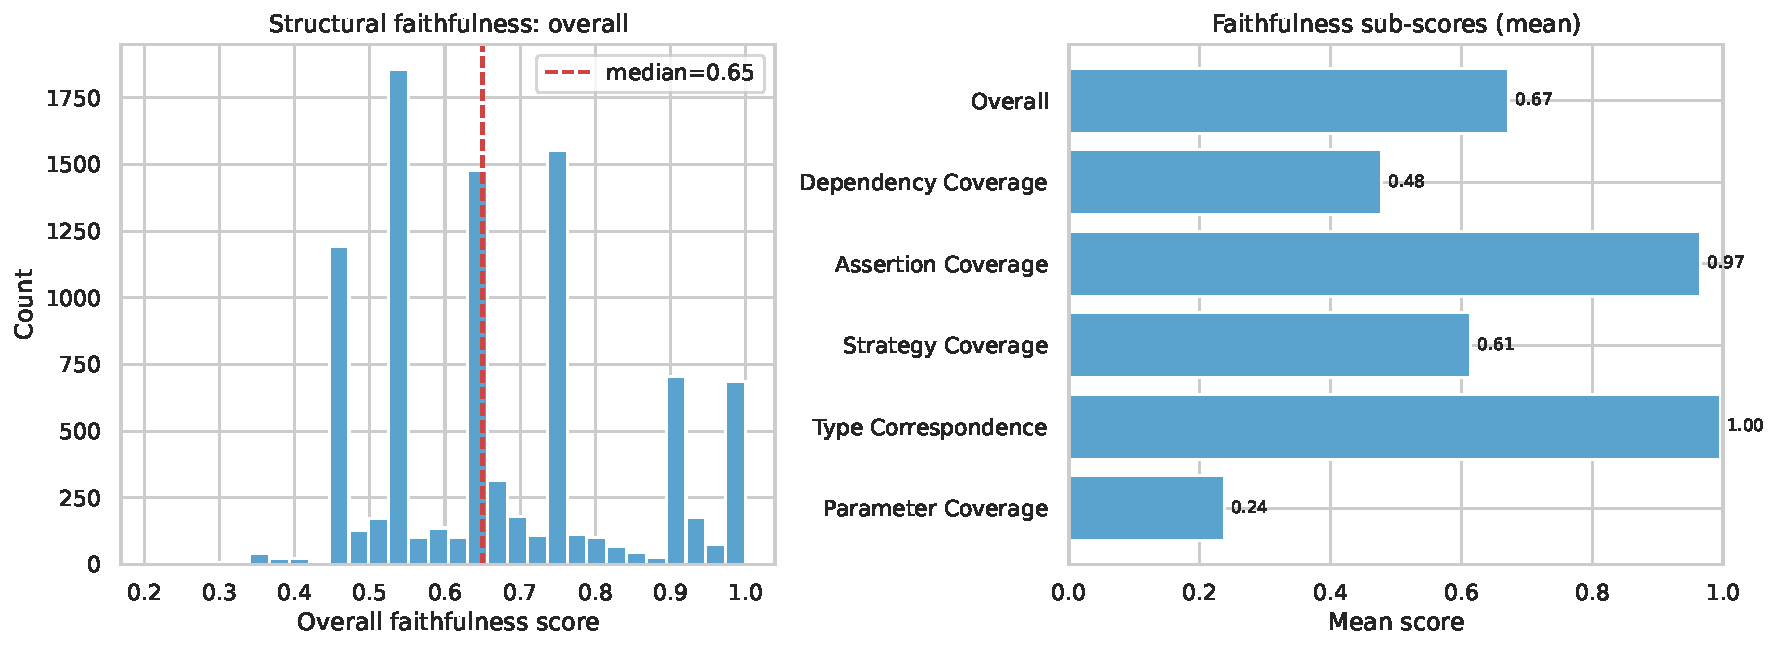
\includegraphics[width=\linewidth]{figs/structural_faithfulness.pdf}
  \caption{Structural faithfulness: distribution of the overall composite score (left) and mean sub-scores (right).}
  \label{fig:structural_faithfulness}
\end{figure}

In 59\% of samples the agent generated a complete Lean implementation (\texttt{Impl.lean} contains a computable definition, not just a stub); the remaining 41\% use a signature-only placeholder. Structural faithfulness is comparable across both groups (mean 0.67 vs.\ 0.68), confirming that specification quality is largely independent of whether the implementation was recovered.

The generated Lean artifacts span a wide range of complexity (Figure~\ref{fig:lean_complexity}): the median sample contains multiple theorems each requiring an independent proof, and the \texttt{sorry} count tracks the theorem count closely, as expected from our pipeline design.

\begin{figure}[t]
  \centering
  
\includegraphics[width=\linewidth]{figs/lean_complexity.pdf}
  \caption{Lean output complexity: total lines (left), theorems per sample (center), and \texttt{sorry} placeholders per sample (right). Tail counts and maxima shown in axis labels.}
  \label{fig:lean_complexity}
\end{figure}

Per-sample pipeline cost is right-skewed (Figure~\ref{fig:pipeline_cost}): most samples compile within a few agent turns, but a tail of difficult translations requires many repair iterations before the Lean LSP reports success or the budget is exhausted.

\begin{figure}[t]
  \centering
  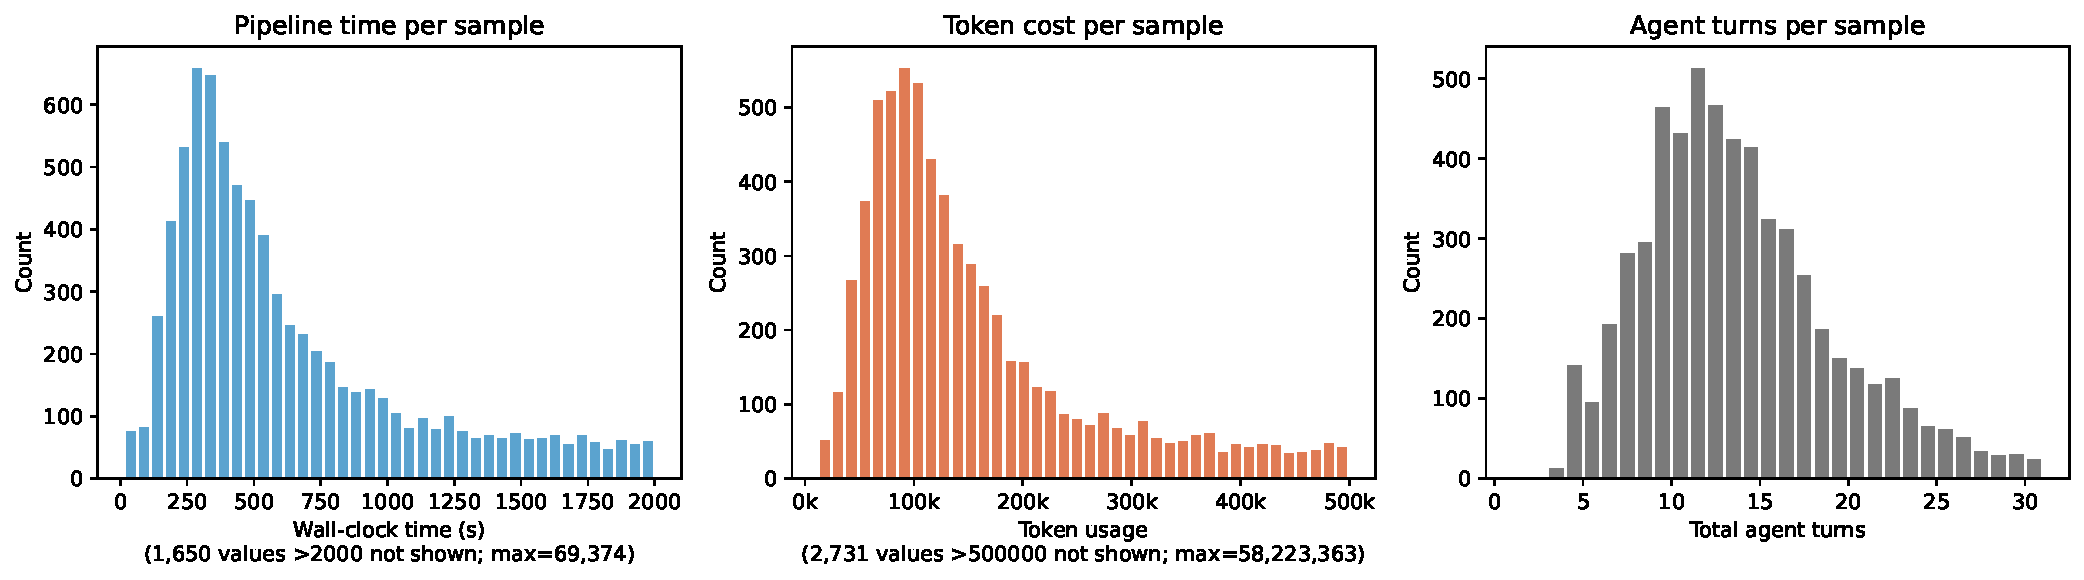
\includegraphics[width=\linewidth]{figs/pipeline_cost.pdf}
  \caption{Pipeline cost per sample: wall-clock time (left), token usage (center), and agent turns (right). Tail counts and maxima shown in axis labels.}
  \label{fig:pipeline_cost}
\end{figure}

\subsection{Difficulty Grading}

Each sample is graded for proof difficulty by Claude Haiku 4.5, which assigns a binary label (\emph{easy} or \emph{hard}) along with a confidence score. Figure~\ref{fig:difficulty_distribution} shows the resulting split and the distribution of grader confidence. The benchmark contains a substantial proportion of both easy and hard problems, and the grader expresses high confidence for the majority of assessments. Difficulty is estimated here as a \textit{prediction}, where we ask the grader to predict whether or not a language model agent would be able to complete the proofs successfully (considering the problem "hard" if haiku thinks not, and "easy" if haiku thinks yes). 

\begin{figure}[t]
  \centering
  
\includegraphics[width=\linewidth]{figs/difficulty_distribution.pdf}
  \caption{Difficulty distribution: easy vs.\ hard counts (left) and grader confidence distribution (right). $n$ shown in title.}
  \label{fig:difficulty_distribution}
\end{figure}

Figure~\ref{fig:difficulty_vs_faithfulness} examines the relationship between difficulty and two output characteristics: structural faithfulness and Lean output size. Hard problems tend to produce longer Lean outputs, consistent with the intuition that more complex source PBTs lead to more elaborate formalizations and more challenging proofs.

\begin{figure}[t]
  \centering
  
\includegraphics[width=\linewidth]{figs/difficulty_vs_faithfulness.pdf}
  \caption{Difficulty vs.\ output characteristics: overall faithfulness (left) and total Lean lines (right), stratified by difficulty.}
  \label{fig:difficulty_vs_faithfulness}
\end{figure}

\subsection{Baselines}

\begin{figure}[t]
  
\includegraphics[width=\linewidth]{figs/baselines_prove_rate.pdf}
  \caption{baseline prove rate}
\end{figure}

We evaluate two frontier models (Claude Sonnet~4.6 and GPT~5.4) on 100 randomly sampled easy problems and 100 hard problems (difficulty as defined in \Secr{results}). Each model has access to the Lean LSP via MCP tools and is scored on two metrics: a binary \emph{proved} flag (zero \texttt{sorry} remaining and \texttt{lake build} succeeds) and \emph{partial credit} (fraction of \texttt{sorry} placeholders removed, clamped to $[0,1]$).

\begin{figure}[t]
  
\includegraphics[width=\linewidth]{figs/baselines_cost.pdf}
  \caption{Compute cost per sample for each baseline run: wall-clock time (left) and token usage (right), summed across all attempts for $k>1$ runs. Box plots show median, IQR, and $1.5\times$IQR whiskers.}
  \label{fig:baselines_cost}
\end{figure}
